\documentclass[12pt, a4paper]{book}

\usepackage[T1]{fontenc}
\usepackage[utf8]{inputenc}
\usepackage[charter, cal=cmcal]{mathdesign}
\usepackage[scaled=0.92]{helvet}
\usepackage{geometry}
\geometry{a4paper, top=30mm, bottom=30mm, inner=32mm, outer=25mm, marginparwidth=18mm}

\usepackage{amsmath, amsthm}
\usepackage[version=4]{mhchem}
\usepackage{graphicx}
\usepackage{xcolor}
\usepackage{tikz}
\usetikzlibrary{arrows.meta, shapes.geometric, positioning, calc, backgrounds}
\usepackage{pgfplots}
\pgfplotsset{compat=1.18}
\usepackage{tcolorbox}
\tcbuselibrary{skins, breakable, theorems}
\usepackage{titlesec}
\usepackage{fancyhdr}
\usepackage{enumitem}
\usepackage{booktabs}
\usepackage{array}
\usepackage{parskip}
\usepackage{siunitx}
\usepackage[colorlinks=true, linkcolor=BrickRed,
            urlcolor=NavyBlue, citecolor=ForestGreen]{hyperref}

% ── Colours (Journey 2 — charcoal / royal blue) ────────────────────────────────
\definecolor{JourneyColor}{HTML}{0F172A}
\definecolor{ModuleColor}{HTML}{2563EB}
\definecolor{PuzzleColor}{HTML}{D97706}
\definecolor{DiscoveryColor}{HTML}{3B82F6}
\definecolor{WarningColor}{HTML}{991B1B}
\definecolor{ProblemColor}{HTML}{6B21A8}
\definecolor{ReflectColor}{HTML}{0D9488}
\definecolor{HistoryColor}{HTML}{78350F}

% ── Boxes ─────────────────────────────────────────────────────────────────────
\newtcolorbox{puzzlebox}[1][]{enhanced,breakable,
  colback=PuzzleColor!6,colframe=PuzzleColor,fonttitle=\bfseries\sffamily,
  title={The Puzzle},attach boxed title to top left={yshift=-2mm,xshift=6mm},
  boxed title style={colback=PuzzleColor},borderline west={3pt}{0pt}{PuzzleColor},#1}

\newtcolorbox{discoverybox}[1][]{enhanced,breakable,
  colback=DiscoveryColor!8,colframe=DiscoveryColor,fonttitle=\bfseries\sffamily,
  title={Discovery},attach boxed title to top left={yshift=-2mm,xshift=6mm},
  boxed title style={colback=DiscoveryColor},borderline west={3pt}{0pt}{DiscoveryColor},#1}

\newtcolorbox{problembox}[1][]{enhanced,breakable,
  colback=ProblemColor!5,colframe=ProblemColor,fonttitle=\bfseries\sffamily,
  title={Problems},attach boxed title to top left={yshift=-2mm,xshift=6mm},
  boxed title style={colback=ProblemColor},borderline west={3pt}{0pt}{ProblemColor},#1}

\newtcolorbox{deepbox}[1][]{enhanced,breakable,
  colback=JourneyColor!5,colframe=JourneyColor,fonttitle=\bfseries\sffamily,
  title={Deep Problems},attach boxed title to top left={yshift=-2mm,xshift=6mm},
  boxed title style={colback=JourneyColor},borderline west={4pt}{0pt}{JourneyColor},#1}

\newtcolorbox{historybox}[1][]{enhanced,breakable,
  colback=HistoryColor!7,colframe=HistoryColor!60,fonttitle=\bfseries\sffamily\small,
  title={Historical Note},attach boxed title to top left={yshift=-2mm,xshift=6mm},
  boxed title style={colback=HistoryColor!80},#1}

\newtcolorbox{reflectionbox}[1][]{enhanced,breakable,
  colback=ReflectColor!6,colframe=ReflectColor,fonttitle=\bfseries\sffamily,
  title={Reflection},attach boxed title to top left={yshift=-2mm,xshift=6mm},
  boxed title style={colback=ReflectColor},borderline west={3pt}{0pt}{ReflectColor},#1}

\newtcolorbox{namedconcept}[2][]{enhanced,
  colback=ModuleColor!6,colframe=ModuleColor,fonttitle=\bfseries\sffamily\large,
  title={#2},attach boxed title to top left={yshift=-2mm,xshift=6mm},
  boxed title style={colback=ModuleColor},#1}

% ── Section formatting ────────────────────────────────────────────────────────
\titleformat{\chapter}[display]
  {\normalfont\sffamily\huge\bfseries\color{JourneyColor}}
  {\textcolor{JourneyColor!60}{\chaptertitlename\ \thechapter}}{10pt}{\Huge}
  [\vspace{2pt}\textcolor{JourneyColor}{\titlerule[1.5pt]}]
\titleformat{\section}
  {\normalfont\sffamily\Large\bfseries\color{ModuleColor}}
  {\thesection}{1em}{}[\textcolor{ModuleColor!40}{\titlerule[0.6pt]}]
\titleformat{\subsection}
  {\normalfont\sffamily\large\bfseries\color{JourneyColor!80}}{\thesubsection}{1em}{}
\titleformat{\subsubsection}
  {\normalfont\sffamily\normalsize\bfseries}{\thesubsubsection}{1em}{}

\pagestyle{fancy}
\fancyhf{}
\fancyhead[LE]{\small\sffamily\textcolor{JourneyColor}{\leftmark}}
\fancyhead[RO]{\small\sffamily\textcolor{ModuleColor}{\rightmark}}
\fancyfoot[C]{\small\thepage}
\renewcommand{\headrulewidth}{0.4pt}

\newcommand{\newterm}[1]{\textit{\textcolor{DiscoveryColor}{#1}}}
\newcommand{\important}[1]{\textcolor{ModuleColor}{\textbf{#1}}}

\begin{document}

\setcounter{chapter}{1}
\chapter[Journey 2 --- Physical Computation (Silicon to Gate)]
        {Journey Two\\[8pt]
         \textcolor{ModuleColor}{\large Physical Computation (Silicon to Gate)}}
\setcounter{section}{3}

\section{Module 2.4 --- Processor Architecture and Memory Hierarchies}
\label{sec:mod2.4}

\subsection*{Motivation}

We mastered in Module 2.3 how combinational blocks process binary bits and how cross-coupled feedback loops construct latches and flip-flops for memory.
Now, we connect these components to build the complete architecture of a computer processor.

The core of a computer is the CPU, which decodes and executes instructions in continuous fetch-decode-execute cycles.
However, processor performance faces a major hardware bottleneck: the **Memory Wall**.
While processor logic speeds have scaled exponentially to the gigahertz range, the speed of main memory (DRAM) has scaled much slower.
Accessing main memory can require hundreds of CPU clock cycles, leaving the processor idle.
This module explores how memory hierarchies (registers, SRAM caches, and DRAM) utilize the spatial and temporal locality of programs to bridge this latency gap, enabling high-speed execution.

\subsection{The Memory Wall}

We analyze the latency gap between processing logic and main memory.

\begin{puzzlebox}
\textbf{The Latency Bottleneck.}

Consider a processor operating at a clock frequency of $f = \SI{4.0}{GHz}$ (1 clock cycle $= \SI{0.25}{ns}$).
* Reading from a local register takes $< 1$ clock cycle ($< \SI{0.25}{ns}$).
* Reading from the main off-chip memory (DRAM) takes $\approx \SI{50}{ns}$ ($\approx 200$ clock cycles).
\begin{enumerate}[label=(\alph*), leftmargin=*]
  \item Suppose a program executes a sequence of instructions where $20\%$ of the instructions must read a data value from main memory.
        If the processor has no cache, and must wait for main memory on every data access, calculate the average clock cycles per instruction (CPI) if the base execution CPI is 1.0.
        What percentage of its time does the CPU spend completely idle, doing no work?
  \item To solve this, we place a small, fast memory called a **Cache** on the same chip as the CPU.
        If the cache has a hit time of 1 clock cycle, and a **Hit Rate** of $95\%$ (meaning $95\%$ of the time the data is found in the cache, and only $5\%$ of the time we must fetch it from main memory), calculate the Average Memory Access Time (AMAT) in clock cycles:
        \[
          \text{AMAT} \;=\; t_{\text{hit}} + (1 - \text{Hit Rate}) \cdot t_{\text{penalty}},
        \]
        where $t_{\text{penalty}} = 200$ cycles.
  \item Explain why a tiny change in the cache hit rate (e.g. from $95\%$ to $90\%$) has a massive impact on the overall speed of the processor.
\end{enumerate}
\end{puzzlebox}

\subsection{SRAM vs. DRAM Cell Physical Duality}

We study the physical chemistry and circuit designs that distinguish cache memory from main memory.

\begin{explobox}
A computer's memory hierarchy uses different hardware cell designs:
* **SRAM (Static RAM):** Used for on-chip caches. It uses the 6-transistor (6T) cross-coupled inverter loop explored in Module 2.3.
* **DRAM (Dynamic RAM):** Used for off-chip main memory. It uses a **1-transistor 1-capacitor (1T-1C)** cell:
\begin{center}
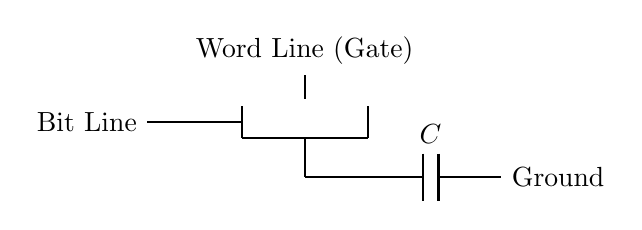
\begin{tikzpicture}[scale=1.0]
  % DRAM cell schematic
  \draw[thick] (0,1.5) -- (0,1.8) node[above] {Word Line (Gate)};
  \draw[thick] (-0.8,1.0) -- (0.8,1.0);
  \draw[thick] (-0.8,1.4) -- (-0.8,1.0);
  \draw[thick] (0.8,1.4) -- (0.8,1.0);
  \draw[thick] (0,1.0) -- (0,0.5);
  \draw[thick] (-0.8,1.2) -- (-2.0,1.2) node[left] {Bit Line};
  
  % Capacitor
  \draw[thick] (0,0.5) -- (1.5,0.5);
  \draw[thick] (1.5,0.8) -- (1.5,0.2);
  \draw[thick] (1.7,0.8) -- (1.7,0.2);
  \draw[thick] (1.7,0.5) -- (2.5,0.5) node[right] {Ground};
  \node[above] at (1.6,0.8) {$C$};
\end{tikzpicture}
\end{center}
\begin{enumerate}[label=(\alph*), leftmargin=*]
  \item Explain why DRAM is much cheaper and denser (packing more bits per unit area of silicon) than SRAM. (Consider the transistor count per cell).
  \item The storage capacitor in a DRAM cell is microscopic, carrying a charge of only a few femtocoulombs.
        Since the access transistor leaks a small subthreshold current (from Module 2.1), this stored charge leaks away over time.
        Explain why DRAM must be periodically **refreshed** (every few milliseconds) by reading and rewriting the data, whereas SRAM holds its data indefinitely as long as power is applied.
  \item Why does this refresh cycle cause DRAM to consume significant power even when the computer is completely idle?
\end{enumerate}
\end{explobox}

\subsection{Principles of Locality}

We study the software behavioral patterns that make cache hierarchies effective.

\begin{explobox}
Caches work because computer programs exhibit the **Principle of Locality**:
* **Temporal Locality:** If a program accesses a memory location, it is highly likely to access the same location again soon.
* **Spatial Locality:** If a program accesses a memory location, it is highly likely to access nearby locations soon.
\begin{enumerate}[label=(\alph*), leftmargin=*]
  \item Consider the following code that sums elements of a 2D array of size $1000 \times 1000$:
        * **Loop 1 (Row-Major):**
          \begin{verbatim}
          for (int i = 0; i < 1000; i++)
              for (int j = 0; j < 1000; j++)
                  sum += A[i][j];
          \end{verbatim}
        * **Loop 2 (Column-Major):**
          \begin{verbatim}
          for (int j = 0; j < 1000; j++)
              for (int i = 0; i < 1000; i++)
                  sum += A[i][j];
          \end{verbatim}
        Recall that arrays are stored in row-major order (consecutive memory locations hold `A[i][0]`, `A[i][1]`, etc.).
        Explain why Loop 1 runs significantly faster than Loop 2 on a processor with a cache, even though both loops execute the exact same number of additions.
  \item When a cache miss occurs, the processor does not fetch just the single requested byte from DRAM. It fetches a contiguous block of memory called a **Cache Line** (typically 64 bytes).
        How does this cache line design exploit spatial locality?
\end{enumerate}
\end{explobox}

\newpage

% ─── Section: Discovery ──────────────────────────────────────────────────────
\section{Part 3 --- Discovery}

\begin{discoverybox}
\textbf{What have we built?}

\textbf{First.} The Von Neumann architecture divides the computer into a processing unit (CPU) and memory, linked by a shared bus.

\textbf{Second.} The Memory Wall is the latency gap between fast processing logic (nanoseconds) and slow main memory DRAM (tens of nanoseconds).

\textbf{Third.} Caches exploit the principles of temporal and spatial locality to keep active data in fast, on-chip SRAM cells, hiding DRAM latency.

\textbf{Fourth.} SRAM uses a 6T cell to hold state statically without leaking. DRAM uses a 1T-1C cell to achieve high density, but requires periodic refresh cycles because the charge leaks.
\end{discoverybox}

\newpage

% ─── Section: Naming Concepts ────────────────────────────────────────────────
\section{Part 4 --- What This Is Called}

\begin{namedconcept}{Processor and Cache parameters}
* **Von Neumann Architecture:** A computer architecture where instruction data and program data share the same physical memory space and bus.
* **SRAM:** Static Random-Access Memory. Fast, low-density, 6-transistor memory.
* **DRAM:** Dynamic Random-Access Memory. Dense, high-latency, 1-transistor 1-capacitor memory.
* **Average Memory Access Time (AMAT):** The average time required to perform a memory access, accounting for cache hit and miss rates.
* **Temporal Locality:** The tendency of a program to reuse recently accessed memory locations.
* **Spatial Locality:** The tendency of a program to access memory locations that are physically close to recently accessed locations.
\end{namedconcept}

\newpage

% ─── Section: Solved Exercises ───────────────────────────────────────────────
\section{Part 5 --- Solved Exercises}

\begin{problembox}
\begin{enumerate}[label=\textbf{E\arabic*.}]
  \item \textbf{Calculating Cache Address Decoding.}
  
        A direct-mapped cache has a total size of $64$ KB ($64 \times 1024 = 65,536$ bytes) with a cache line size of $64$ bytes. The processor uses $32$-bit physical addresses.
        Show how the 32-bit address is split into Tag, Index, and Offset fields to access the cache.
        
        \textbf{Solution:}
        In a direct-mapped cache:
        * The **Offset** bits select the specific byte within a cache line.
        * The **Index** bits select the specific cache line row.
        * The **Tag** bits are stored in the cache directory to verify if the cached block matches the requested address.
        
        1. **Calculate the Offset bits:**
           The cache line size is 64 bytes.
           The number of bits required to address 64 bytes is:
           \[
             \text{Offset bits} \;=\; \log_2(64) \;=\; 6 \text{ bits}.
           \]
           Thus, the lowest 6 bits (bits 0 to 5) of the address represent the Offset.
           
        2. **Calculate the Index bits:**
           The total size of the cache is 64 KB, and each line is 64 bytes.
           The total number of cache lines (rows) is:
           \[
             \text{Number of lines} \;=\; \frac{\text{Total Cache Size}}{\text{Line Size}} \;=\; \frac{64 \times 1024 \text{ bytes}}{64 \text{ bytes}} \;=\; 1024 \text{ lines}.
           \]
           The number of bits required to uniquely select one of 1024 lines is:
           \[
             \text{Index bits} \;=\; \log_2(1024) \;=\; 10 \text{ bits}.
           \]
           Thus, the next 10 bits (bits 6 to 15) of the address represent the Index.
           
        3. **Calculate the Tag bits:**
           The remaining bits of the 32-bit address represent the Tag.
           \[
             \text{Tag bits} \;=\; 32 - (\text{Index bits} + \text{Offset bits}) \;= \; 32 - (10 + 6) \;=\; 32 - 16 \;=\; 16 \text{ bits}.
           \]
           Thus, the upper 16 bits (bits 16 to 31) of the address represent the Tag.
           
        Therefore, the 32-bit address is divided as:
        * **Tag:** Bits 31 to 16 (16 bits)
        * **Index:** Bits 15 to 6 (10 bits)
        * **Offset:** Bits 5 to 0 (6 bits)
        
  \item \textbf{Average Memory Access Time (AMAT) Analysis.}
  
        A processor has a primary L1 cache with a hit time of 1 clock cycle.
        The local L1 miss rate is $4.0\%$.
        If an L1 miss occurs, the processor checks a larger L2 cache, which has a hit time of 8 clock cycles and a local miss rate of $15\%$.
        If both L1 and L2 miss, the processor must access DRAM, which takes an additional 200 clock cycles.
        Calculate the overall AMAT of the processor.
        
        \textbf{Solution:}
        For a multi-level cache hierarchy, the AMAT is calculated recursively:
        \[
          \text{AMAT} \;=\; t_{\text{hit, L1}} + \text{Miss Rate}_{\text{L1}} \cdot \text{AMAT}_{\text{L2}},
        \]
        where the access time of the L2 sub-hierarchy is:
        \[
          \text{AMAT}_{\text{L2}} \;=\; t_{\text{hit, L2}} + \text{Miss Rate}_{\text{L2}} \cdot t_{\text{DRAM}}.
        \]
        Here:
        * $t_{\text{hit, L1}} = 1$ cycle.
        * $\text{Miss Rate}_{\text{L1}} = 0.04$.
        * $t_{\text{hit, L2}} = 8$ cycles.
        * $\text{Miss Rate}_{\text{L2}} = 0.15$.
        * $t_{\text{DRAM}} = 200$ cycles.
        
        First, calculate the average access time for an L2 query:
        \[
          \text{AMAT}_{\text{L2}} \;=\; 8 + (0.15 \times 200) \;=\; 8 + 30 \;=\; 38 \text{ cycles}.
        \]
        Now, substitute this back into the L1 equation:
        \[
          \text{AMAT} \;=\; 1 + (0.04 \times 38) \;=\; 1 + 1.52 \;=\; 2.52 \text{ cycles}.
        \]
        Thus, the overall Average Memory Access Time is $2.52$ clock cycles.
        Note that this is close to the L1 hit time of 1 cycle, showing that the cache hierarchy successfully hides the 200-cycle DRAM latency.
\end{enumerate}
\end{problembox}

\newpage

% ─── Section: Problems ───────────────────────────────────────────────────────
\section{Part 6 --- Problems}

\begin{problembox}
\begin{enumerate}[label=\textbf{P\arabic*.}]
  \item \textbf{Amdahl's Law and Memory Bottlenecks.}
  
        A processor spends $35\%$ of its execution cycles waiting for memory requests.
        Suppose a cache architect designs a new L3 cache that accelerates memory access times by a factor of 4.
        \begin{enumerate}[label=(\alph*)]
          \item State Amdahl's Law for calculating speedup:
                \[
                  \text{Speedup} \;=\; \frac{1}{(1 - f_{\text{enhanced}}) + \frac{f_{\text{enhanced}}}{S}},
                \]
                where $f_{\text{enhanced}}$ is the fraction of time affected and $S$ is the speedup factor.
          \item Calculate the overall processor speedup achieved by this L3 cache.
          \item If the cache could accelerate memory accesses infinitely ($S \to \infty$), calculate the theoretical maximum speedup limit.
                Why does this demonstrate the structural limit of the "Von Neumann Bottleneck"?
        \end{enumerate}

  \item **Direct-Mapped vs. Set-Associative Caches.**
  
        In a direct-mapped cache, each memory address maps to exactly one cache line, which can cause **conflict misses** if a program accesses two different variables that map to the same row.
        To solve this, we use a **2-Way Set-Associative cache**, where each index maps to a *set* containing two cache lines.
        \begin{enumerate}[label=(\alph*)]
          \item Consider a cache of size 64 KB with 64-byte cache lines.
                If we change the design from direct-mapped to 2-way set-associative, how does the number of sets change?
          \item Calculate the new number of Index and Tag bits for a 32-bit physical address.
          \item A set-associative cache requires a replacement policy (such as Least Recently Used, LRU) to decide which line to evict when a set is full.
                Explain how this policy uses temporal locality to make eviction choices.
        \end{enumerate}
\end{enumerate}
\end{problembox}

\newpage

% ─── Section: Deep Problems ──────────────────────────────────────────────────
\section{Part 7 --- Deep Problems}

\begin{deepbox}
\begin{enumerate}[label=\textbf{D\arabic*.}]
  \item \textbf{The Three C's of Cache Misses.}
  
        Cache misses are classified into three types:
        1. **Compulsory (Cold) Misses:** The first access to a block, which has never been in the cache.
        2. **Capacity Misses:** Occur when the cache cannot contain all the blocks needed during program execution.
        3. **Conflict Misses:** Occur when multiple blocks map to the same set, causing evictions despite the cache having vacant lines elsewhere.
        
        \begin{enumerate}[label=(\alph*)]
          \item For each of the following design modifications, analyze how it shifts the balance between the three types of misses:
                * Design A: Doubling the total cache size (keeping block size and associativity constant).
                * Design B: Increasing the associativity (e.g., from direct-mapped to 8-way, keeping cache size and block size constant).
                * Design C: Doubling the block size (cache line size) from 64 to 128 bytes (keeping total cache size and associativity constant).
          \item In Design C, explain why doubling the block size decreases compulsory misses (due to spatial locality) but can *increase* capacity misses if the cache gets filled with unused bytes. (This is **cache pollution**).
        \end{enumerate}

  \item \textbf{SRAM Read/Write Noise Margin Limits.}
  
        We model a 6T SRAM cell containing two cross-coupled CMOS inverters and two access transistors connected to the Bit Lines ($BL$ and $\overline{BL}$).
        During a write operation, the bit lines are driven to $V_{DD}$ and Ground, and the access transistors must force the internal loop to flip its state.
        \begin{enumerate}[label=(\alph*)]
          \item For a write to be successful, the access transistor must be strong enough to overpower the pull-up pMOS transistor of the inverter that is holding the node high.
                Explain why this requires the access transistor to have a larger width-to-length ratio ($W/L$) than the pull-up pMOS.
          \item Write down the three conflicting design constraints in a 6T SRAM cell:
                1. Read Stability (requires strong pull-down nMOS relative to access transistor).
                2. Write Ability (requires strong access transistor relative to pull-up pMOS).
                3. Leakage minimization.
                Show why sizing these 6 transistors represents a critical optimization challenge in nano-scale fabrication nodes.
        \end{enumerate}
\end{enumerate}
\end{deepbox}

\newpage

% ─── Section: Reflection ─────────────────────────────────────────────────────
\section{Part 8 --- Reflection}

\begin{reflectionbox}
\textbf{Conceptual Reflection}

Consider the following questions:
\begin{enumerate}
  \item **On the Hierarchy of Scale:** Registers are fast and small; DRAM is slow and large. This hierarchy mirrors the physical universe: small structures operate at high frequencies, while large structures have long relaxation times. Why is this scaling of size and time a universal property of physical and logical networks?
  \item **On Locality as Program Intent:** Caches only work because human programmers write code with structured loops and sequential arrays (locality). If a program accessed memory locations completely at random, the cache hit rate would drop to zero, and the processor would grind to a halt. Is the speed of our computers a consequence of the orderliness of human thought?
  \item **On the Von Neumann Bottleneck:** Sharing a single bus for instructions and data limits throughput. The human brain, by contrast, co-locates memory and processing inside the same neural junctions (synapses). How would computer architectures change if we abandoned the Von Neumann separation and co-located logic and storage within the same silicon cells?
\end{enumerate}
\end{reflectionbox}

\medskip
\noindent\textbf{Looking back at Journey 2.}
You have traversed the physical foundations of computation:
* **Module 2.1:** Doping chemistry, MOSFET structures, inversion layers, and scaling limits.
* **Module 2.2:** Pull-up/pull-down CMOS networks, propagation delay, and switching power kinetics.
* **Module 2.3:** Combinational adders/multiplexers, and sequential Latches/Flip-Flops.
* **Module 2.4:** Processor execution loop datapath, SRAM vs. DRAM cell physical dualities, and cache hierarchies.

This completes Journey 2, providing the complete physical and architectural foundation of computer processors. You are now ready to proceed to: **Computation Journey 3 --- Automata, Complexity, and the Limits of Computation**.

\vspace{1.4cm}
\begin{center}
{\color{JourneyColor}\rule{0.5\linewidth}{0.8pt}}\\[6pt]
{\small\color{JourneyColor}\textit{End of Journey 2 --- Physical Computation (Silicon to Gate)}}\\[4pt]
{\small\color{JourneyColor}You have completed the hardware architecture track. Continue to: \textbf{Computation Journey 3 --- Automata, Complexity, and the Limits of Computation}}\\[6pt]
{\color{JourneyColor}\rule{0.5\linewidth}{0.8pt}}
\end{center}

\end{document}
